\chapter{基于先验地图约束的轴向-非轴向分解与融合定位方法}

\section{引言}

矿井巷道环境属于典型的卫星导航拒止场景，车辆位姿估计主要依赖激光点云、惯性信息以及已有先验地图。与地面开放环境相比，矿井巷道具有显著的狭长结构特征，沿巷道延伸方向的几何形态重复性较强，而横断面方向的结构边界相对稳定。这种方向性差异使得点云与先验地图之间的配准约束呈现出明显的不均衡性，若仍采用统一权重处理不同方向上的观测信息，则容易在局部结构退化、匹配初值偏差或观测质量波动时产生定位不稳定现象。

针对上述问题，本章提出一种基于先验地图约束的轴向-非轴向分解与融合定位方法，整体流程如图~\ref{fig:ch4_localization_framework} 所示。
\begin{figure}[htbp]
    \centering
    \IfFileExists{figures/图4.1基于先验体素约束与轴向分解融合的矿井定位总体框架图.drawio.pdf}{
        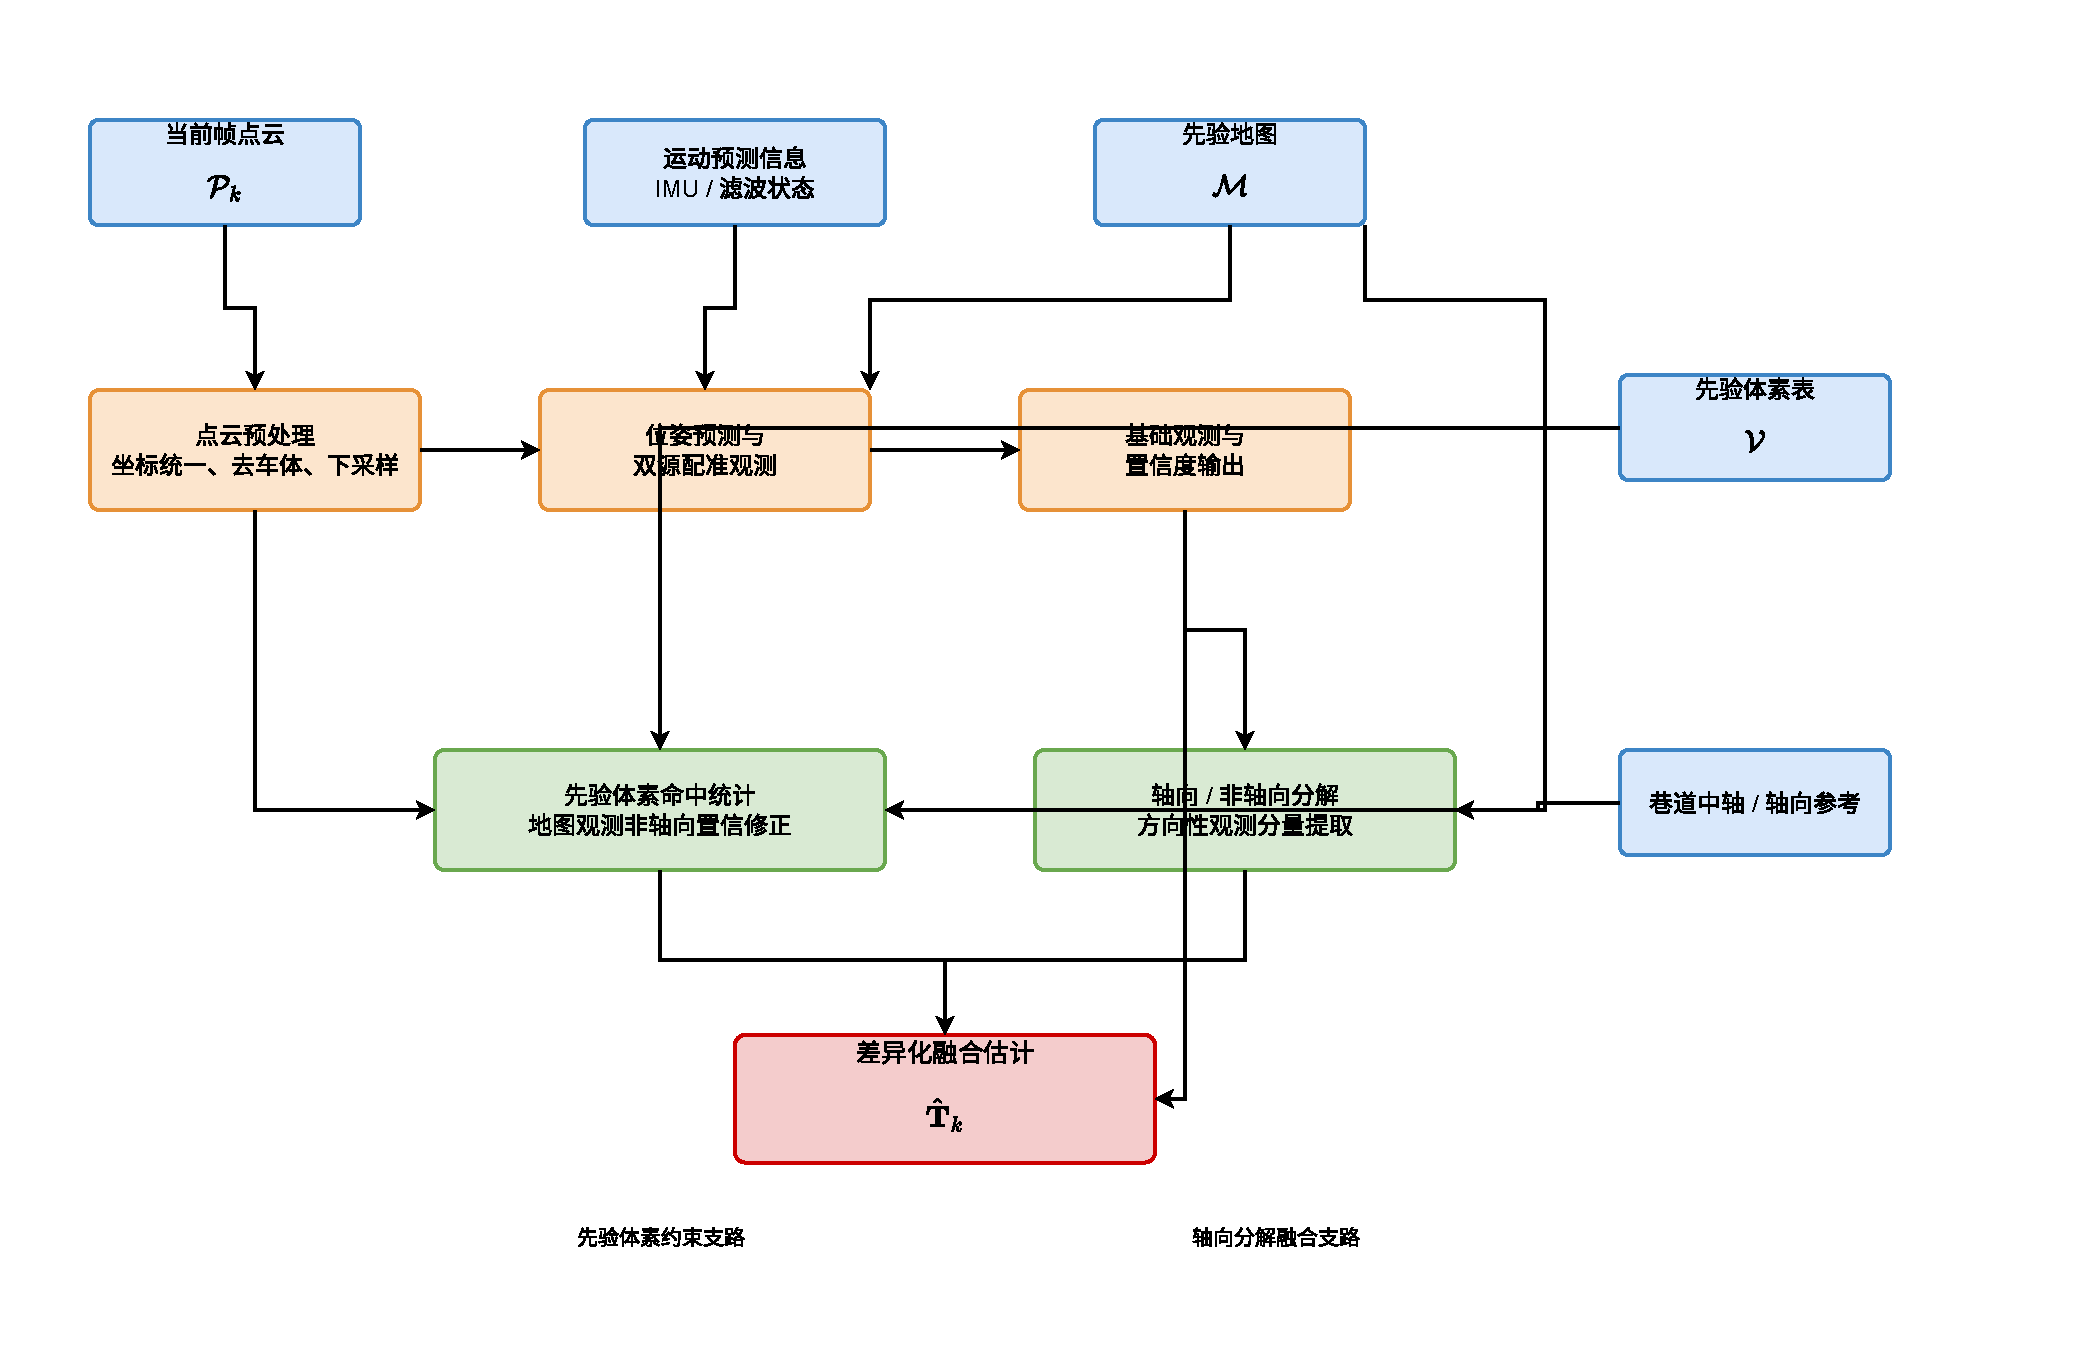
\includegraphics[width=0.98\linewidth]{figures/图4.1基于先验体素约束与轴向分解融合的矿井定位总体框架图.drawio.pdf}
    }{
        \fbox{
            \parbox{0.92\linewidth}{
                \centering
                图4.1 基于先验地图约束的轴向-非轴向分解与融合定位总体框架图占位图\\[4pt]
                当前仓库中仅存在对应的 \texttt{.drawio} 源文件，待导出为 \texttt{.pdf} 后可替换此占位框。
            }
        }
    }
    \caption{基于先验地图约束的轴向-非轴向分解与融合定位总体框架图}
    \label{fig:ch4_localization_framework}
\end{figure}

该方法以当前帧点云、运动预测信息和先验地图为基础，首先构建位姿预测与双源配准观测模块，得到帧间位姿观测、地图位姿观测及其基础置信度；随后，结合巷道中轴信息和先验体素命中统计，分别构建轴向与非轴向方向上的观测分解与约束建模；最后，通过加权融合估计获得当前时刻位姿。通过将先验地图约束、轴向-非轴向观测分解和融合机制共同引入定位过程，能够在保持地图全局约束能力的同时，增强矿井巷道场景下定位结果的稳定性与适应性。

% 建议补图4.1：基于先验地图约束的轴向-非轴向分解与融合定位总体框架图。
% 建议内容：
% 1. 输入端包括：当前帧点云、IMU/预测信息、先验地图、先验体素表、中轴线数据。
% 2. 中间流程包括：帧到地图配准、帧间配准、配准得分置信度计算、先验体素命中统计、
%    中轴投影、轴向/非轴向分解、差异化权重融合。
% 3. 输出端包括：最终位姿估计，以及可选的调试量（map/f2f置信度、轴向与非轴向权重等）。
% 4. 图形风格建议采用流程框图，突出“先验地图约束”和“轴向-非轴向分解与融合”两条核心主线，
%    配准观测框架作为基础支撑模块展示即可。

\section{位姿预测与配准观测模型构建}

为将先验地图约束、轴向-非轴向分解与融合机制统一纳入定位估计过程，本节首先构建位姿预测与双源配准观测模型。整体上，本文采用“惯性预测--帧间配准--地图配准”的递进式观测建模策略：先利用 IMU 运动信息生成当前时刻的初始位姿预测，再依次构建帧间配准观测和地图配准观测，形成由运动先验到局部观测再到全局观测的层级化位姿估计过程。整体流程如图~\ref{fig:ch4_progressive_observation} 所示。

\begin{figure}[htbp]
    \centering
    \IfFileExists{figures/图4.2位姿预测与双源配准观测建模流程图.drawio.pdf}{
        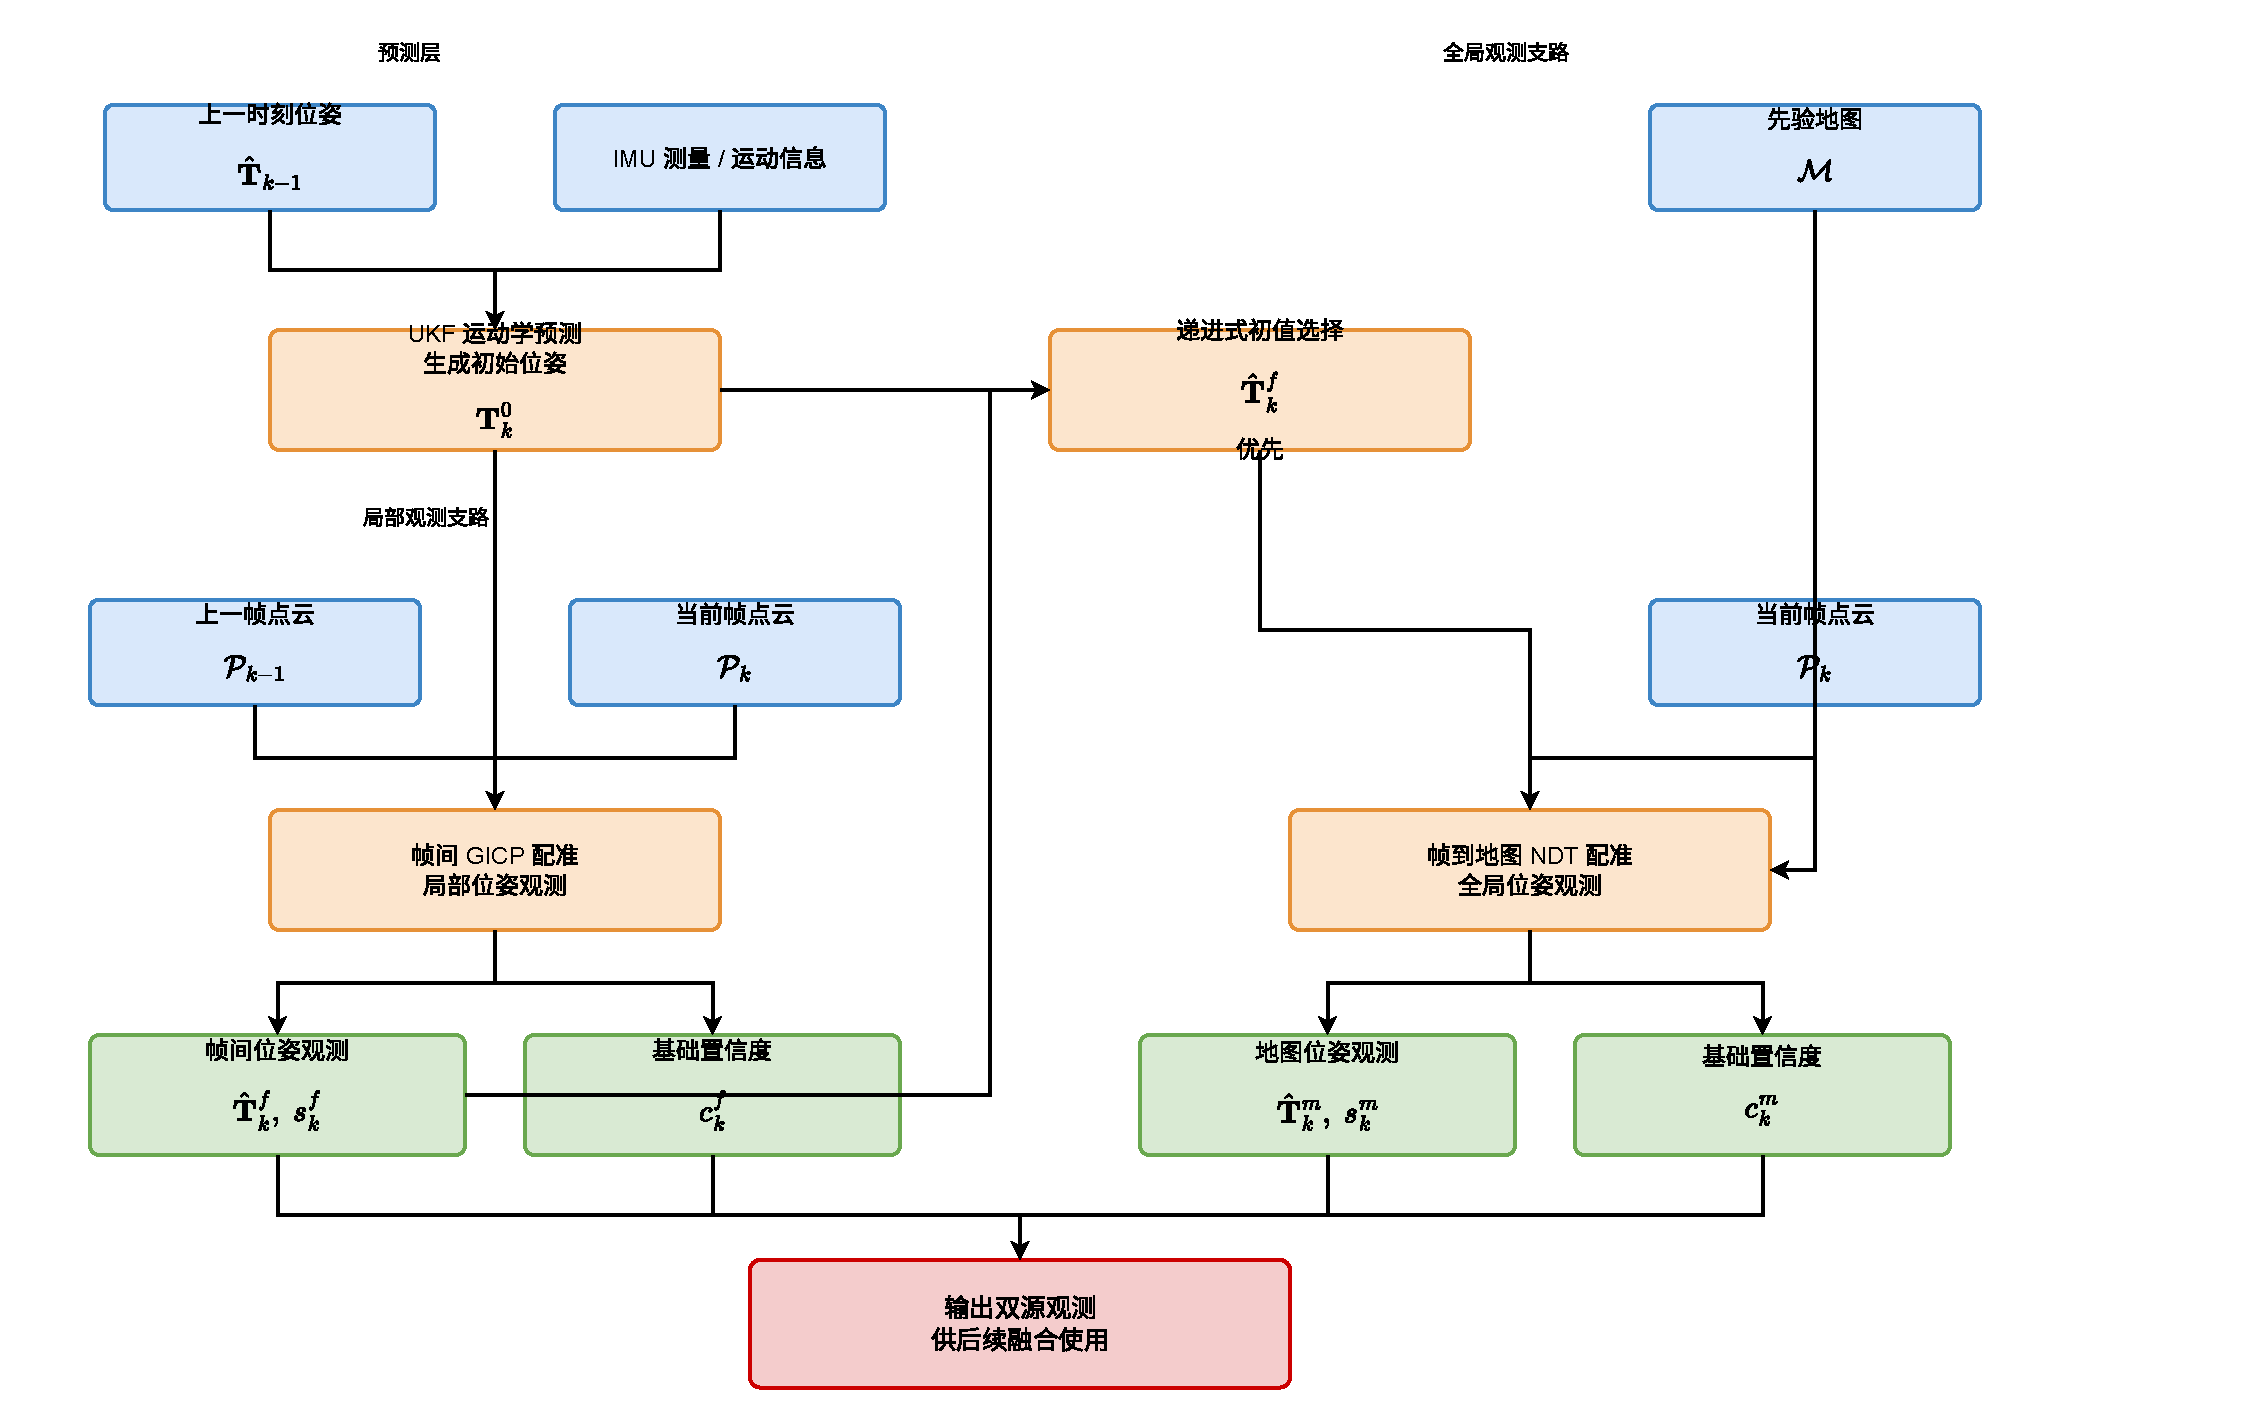
\includegraphics[width=0.98\linewidth]{figures/图4.2位姿预测与双源配准观测建模流程图.drawio.pdf}
    }{
        \fbox{
            \parbox{0.92\linewidth}{
                \centering
                图4.2 位姿预测与双源配准观测建模流程图占位图\\[4pt]
                当前仓库中仅存在对应的 \texttt{.drawio} 源文件，待导出为 \texttt{.pdf} 后可替换此占位框。
            }
        }
    }
    \caption{位姿预测与双源配准观测建模流程图}
    \label{fig:ch4_progressive_observation}
\end{figure}

为兼顾局部运动估计的连续性与全局地图匹配的稳定性，本文在该递进式观测框架中分别构建帧间配准观测和地图配准观测。帧间配准面向时间相邻且重叠度较高的局部点云观测，不直接依赖先验地图，因此在实现层面采用 GICP 的多线程高效实现 Fast-GICP 完成点云配准，而在理论描述上仍按 GICP 的概率配准模型构建局部位姿观测。地图配准面向大规模先验地图，为减弱显式最近邻点对匹配带来的错误对应与局部极值影响，本文采用基于体素高斯分布建模的 NDT 构建全局位姿观测。帧间配准结果优先作为地图配准的初始化位姿，二者分别输出位姿估计和匹配得分，并进一步转换为后续融合所需的观测置信信息。

\subsection{基于 IMU 运动学模型的初始位姿预测}

为提高后续配准过程的收敛稳定性，本文在每次点云观测到来之前首先利用 IMU 测量对系统状态进行先验传播，并在滤波框架中生成当前时刻的初始位姿预测。设时刻 $k$ 的滤波状态向量为：
\begin{equation}
\mathbf{x}_{k}=
\left[
\mathbf{p}_{k}^{\mathrm{T}},
\mathbf{v}_{k}^{\mathrm{T}},
\mathbf{q}_{k}^{\mathrm{T}},
\mathbf{b}_{a,k}^{\mathrm{T}},
\mathbf{b}_{g,k}^{\mathrm{T}}
\right]^{\mathrm{T}}
\end{equation}

其中，$\mathbf{p}_{k}\in \mathbb{R}^{3}$ 表示位置，$\mathbf{v}_{k}\in \mathbb{R}^{3}$ 表示速度，$\mathbf{q}_{k}=[q_{w},q_{x},q_{y},q_{z}]^{\mathrm{T}}$ 表示姿态四元数，$\mathbf{b}_{a,k}$ 与 $\mathbf{b}_{g,k}$ 分别表示加速度计偏置与陀螺仪偏置。由状态向量可进一步得到当前时刻的位姿表示：
\begin{equation}
\mathbf{T}_{k}=
\begin{bmatrix}
\mathbf{R}\left(\mathbf{q}_{k}\right) & \mathbf{p}_{k}\\
\mathbf{0}^{\mathrm{T}} & 1
\end{bmatrix}
\in SE(3)
\end{equation}

设 IMU 控制输入为 $\mathbf{u}_{k}$，则状态传播模型可统一写为：
\begin{equation}
\mathbf{x}_{k}^{-}
=
f\left(\mathbf{x}_{k-1},\mathbf{u}_{k}\right)
\end{equation}

其中，$\mathbf{x}_{k}^{-}$ 表示时刻 $k$ 的先验状态，$\mathbf{u}_{k}$ 表示 IMU 控制输入。设 IMU 坐标系为 $\{I\}$，激光雷达坐标系为 $\{L\}$，二者之间的固定外参变换为：
\begin{equation}
\mathbf{T}_{L}^{I}
=
\begin{bmatrix}
\mathbf{R}_{L}^{I} & \mathbf{t}_{L}^{I}\\
\mathbf{0}^{\mathrm{T}} & 1
\end{bmatrix}
\end{equation}

由于加速度与角速度均属于向量量，其从 IMU 坐标系到激光雷达坐标系的转换仅与旋转外参有关，因此有：
\begin{equation}
\tilde{\mathbf{a}}_{k}
=
\mathbf{R}_{L}^{I}\tilde{\mathbf{a}}_{k}^{I},
\qquad
\tilde{\boldsymbol{\omega}}_{k}
=
\mathbf{R}_{L}^{I}\tilde{\boldsymbol{\omega}}_{k}^{I}
\end{equation}

其中，$\tilde{\mathbf{a}}_{k}^{I}$ 与 $\tilde{\boldsymbol{\omega}}_{k}^{I}$ 分别表示 IMU 原始输出的加速度计与陀螺仪测量，$\tilde{\mathbf{a}}_{k}$ 与 $\tilde{\boldsymbol{\omega}}_{k}$ 表示转换到激光雷达坐标系后的测量值。因此，后续位姿预测与点云配准均在统一坐标系下进行。将 IMU 原始加速度测量和角速度测量转换到激光雷达坐标系后，测量模型可写为：
\begin{equation}
\tilde{\mathbf{a}}_{k}
=
\mathbf{a}_{k}
+\mathbf{b}_{a,k}
+\mathbf{n}_{a,k},
\qquad
\tilde{\boldsymbol{\omega}}_{k}
=
\boldsymbol{\omega}_{k}
+\mathbf{b}_{g,k}
+\mathbf{n}_{g,k}
\end{equation}

其中，$\mathbf{a}_{k}$ 与 $\boldsymbol{\omega}_{k}$ 分别表示激光雷达坐标系下的加速度项和角速度项，$\mathbf{b}_{a,k}$ 与 $\mathbf{b}_{g,k}$ 分别表示对应的零偏项，$\mathbf{n}_{a,k}$ 与 $\mathbf{n}_{g,k}$ 分别表示加速度计和陀螺仪测量噪声。于是，控制输入可写为：
\begin{equation}
\mathbf{u}_{k}
=
\left[
\tilde{\mathbf{a}}_{k}^{\mathrm{T}},
\tilde{\boldsymbol{\omega}}_{k}^{\mathrm{T}}
\right]^{\mathrm{T}}
\end{equation}

其中，$\mathbf{u}_{k}$ 由当前时刻的加速度观测与角速度观测组成。本文在相邻采样间隔内对平移运动采用恒速假设，并对 IMU 偏置采用短时常值近似。设相邻两个传播时刻之间的时间间隔为 $\Delta t_k$，则 UKF 的先验状态传播可写为：
\begin{equation}
\mathbf{p}_{k}^{-}
=
\mathbf{p}_{k-1}
+\mathbf{v}_{k-1}\Delta t_k
\end{equation}

\begin{equation}
\mathbf{v}_{k}^{-}
=
\mathbf{v}_{k-1}
\end{equation}

\begin{equation}
\mathbf{R}_{k}^{-}
=
\mathbf{R}\left(\mathbf{q}_{k-1}\right)
\mathrm{Exp}
\left(
\left(
\tilde{\boldsymbol{\omega}}_{k}-\mathbf{b}_{g,k-1}-\mathbf{n}_{g,k}
\right)
\Delta t_k
\right)
\end{equation}

其中，$\mathrm{Exp}(\cdot)$ 表示从李代数到旋转群的指数映射。加速度计偏置和陀螺仪偏置在相邻采样间隔内近似保持不变，即 $\mathbf{b}_{a,k}^{-}=\mathbf{b}_{a,k-1}$、$\mathbf{b}_{g,k}^{-}=\mathbf{b}_{g,k-1}$。由 $\mathbf{R}_{k}^{-}$ 可等价得到姿态四元数 $\mathbf{q}_{k}^{-}$。

通过上述先验传播过程可构造当前时刻的初始位姿估计 $\mathbf{T}_{k}^{0}$，即：
\begin{equation}
\mathbf{T}_{k}^{0}=
\begin{bmatrix}
\mathbf{R}_{k}^{-} & \mathbf{p}_{k}^{-}\\
\mathbf{0}^{\mathrm{T}} & 1
\end{bmatrix}
\end{equation}

其中，$\mathbf{p}_{k}^{-}$ 与 $\mathbf{R}_{k}^{-}$ 分别表示先验状态中的位置和姿态。

\subsection{基于帧间配准的局部位姿观测建模}

在获得当前时刻的初始预测位姿后，本文首先构建帧间配准观测。本小节的目的不是展开 Fast-GICP 的全部工程实现细节，而是给出后续融合所需的帧间位姿观测 $\hat{\mathbf{T}}_{k}^{f}$ 及其基础置信度 $c_{k}^{f}$ 的构造过程。帧间点云配准在实现层面采用 Fast-GICP，而以下公式仍按 GICP 的概率配准模型进行表述。记当前时刻经坐标统一、车体点剔除及下采样处理后的点云为 $\mathcal{P}_{k}=\{\mathbf{a}_1,\mathbf{a}_2,\dots,\mathbf{a}_N\}$，上一时刻对应点云为 $\mathcal{P}_{k-1}=\{\mathbf{b}_1,\mathbf{b}_2,\dots,\mathbf{b}_M\}$。设上一时刻最终位姿为 $\hat{\mathbf{T}}_{k-1}$，则当前时刻的帧间初始相对位姿可表示为：
\begin{equation}
\Delta \mathbf{T}_{k}^{0}
=
\left(\hat{\mathbf{T}}_{k-1}\right)^{-1}\mathbf{T}_{k}^{0}
\end{equation}

其中，$\mathbf{T}_{k}^{0}$ 为上一小节得到的预测初值。在初始相对位姿 $\Delta \mathbf{T}_{k}^{0}$ 的引导下，采用 K-D 树在目标点云 $\mathcal{P}_{k-1}$ 中为每个源点搜索最近邻，并建立对应点对集合 $\mathcal{C}_{k}=\{(\mathbf{a}_i,\mathbf{b}_i)\}$。其中，$\Delta \mathbf{T}_{k}^{0}=[\mathbf{R}_{\Delta}^{0},\mathbf{t}_{\Delta}^{0}]$。对每个对应点，利用其局部邻域估计结构协方差，即：
\begin{equation}
\mathbf{C}_{i}^{A}
=
\operatorname{Cov}\!\left(\mathcal{N}(\mathbf{a}_i)\right),
\qquad
\mathbf{C}_{i}^{B}
=
\operatorname{Cov}\!\left(\mathcal{N}(\mathbf{b}_i)\right)
\end{equation}

进一步地，可将源点和目标点的局部结构分别建模为高斯分布：
\begin{equation}
\mathbf{a}_i \sim \mathcal{N}\!\left(\hat{\mathbf{a}}_i,\mathbf{C}_{i}^{A}\right),
\qquad
\mathbf{b}_i \sim \mathcal{N}\!\left(\hat{\mathbf{b}}_i,\mathbf{C}_{i}^{B}\right)
\end{equation}

设待求的相对位姿为 $\Delta \mathbf{T}=[\mathbf{R}_{\Delta},\mathbf{t}_{\Delta}]$，则对应点对的变换误差可表示为：
\begin{equation}
\mathbf{d}_i
=
\hat{\mathbf{b}}_i-\left(\mathbf{R}_{\Delta}\hat{\mathbf{a}}_i+\mathbf{t}_{\Delta}\right)
\end{equation}

由高斯分布的可加性可知，$\mathbf{d}_i$ 服从如下分布：
\begin{equation}
\mathbf{d}_i
\sim
\mathcal{N}\!\left(
\mathbf{0},
\mathbf{C}_{i}^{B}+\mathbf{R}_{\Delta}\mathbf{C}_{i}^{A}\mathbf{R}_{\Delta}^{\mathrm{T}}
\right)
\end{equation}

因此，帧间相对位姿的求解可抽象表示为：
\begin{equation}
\Delta \hat{\mathbf{T}}_{k}^{f}
=
\arg \min_{\Delta \mathbf{T}\in SE(3)}
J_{f}\left(\Delta \mathbf{T};\mathcal{P}_{k},\mathcal{P}_{k-1},\Delta \mathbf{T}_{k}^{0}\right)
\end{equation}

其中，$J_{f}(\cdot)$ 表示当前帧点云与上一帧点云之间的配准目标函数。根据最大似然估计，可将该目标函数进一步写为：
\begin{equation}
J_{f}\left(\Delta \mathbf{T}\right)
=
\sum_{i\in \mathcal{C}_{k}}
\mathbf{d}_{i}^{\mathrm{T}}
\left(
\mathbf{C}_{i}^{B}
+
\mathbf{R}_{\Delta}
\mathbf{C}_{i}^{A}
\mathbf{R}_{\Delta}^{\mathrm{T}}
\right)^{-1}
\mathbf{d}_{i}
\end{equation}

其中，$\mathbf{R}_{\Delta}$ 和 $\mathbf{t}_{\Delta}$ 分别表示相对变换 $\Delta \mathbf{T}$ 的旋转与平移分量。上述目标函数本质上是对所有对应点对变换误差的加权马氏距离求和，通过局部协方差对残差进行方向相关的加权，使不同方向上的几何约束强度能够随邻域结构自适应调整。该配准问题可归结为非线性优化问题，在本文所采用的 Fast-GICP 实现中，使用列文伯格-马夸特（Levenberg-Marquardt，LM）方法对上述目标函数进行迭代优化。由相对位姿结果可进一步得到当前时刻的帧间绝对位姿观测：
\begin{equation}
\hat{\mathbf{T}}_{k}^{f}
=
\hat{\mathbf{T}}_{k-1}\Delta \hat{\mathbf{T}}_{k}^{f}
\end{equation}

帧间配准完成后，可进一步计算匹配得分 $s_{k}^{f}$，用于表征当前帧与上一帧之间的配准一致性。设 $\Delta \hat{\mathbf{T}}_{k}^{f}=[\mathbf{R}_{\Delta}^{\ast},\mathbf{t}_{\Delta}^{\ast}]$，则其形式可写为：
\begin{equation}
s_{k}^{f}
=
\frac{1}{N_k}
\sum_{i=1}^{N_k}
\min_{\mathbf{q}\in \mathcal{P}_{k-1}}
\left\|
\mathbf{q}
-\left(
\mathbf{R}_{\Delta}^{\ast}\mathbf{a}_i+\mathbf{t}_{\Delta}^{\ast}
\right)
\right\|_2^2
\end{equation}

其中，$N_k$ 表示参与统计的源点数。匹配得分越小，说明帧间配准结果与目标点云的一致性越高。为将该信息用于后续观测融合，进一步定义帧间观测的基础置信度为：
\begin{equation}
c_{k}^{f}
=
\psi\!\left(s_{k}^{f}\right)
=
\mathrm{clip}
\left(
\frac{s_{\mathrm{bad}}-s_{k}^{f}}{s_{\mathrm{bad}}-s_{\mathrm{good}}},
0,1
\right)
\end{equation}

其中，$\psi(\cdot)$ 表示由匹配得分到置信度的映射函数，$s_{\mathrm{good}}$ 与 $s_{\mathrm{bad}}$ 分别表示匹配得分的优、劣边界，$\mathrm{clip}(x,0,1)$ 表示将变量 $x$ 截断到区间 $[0,1]$ 内。

综上，帧间配准模块输出局部连续位姿观测 $\hat{\mathbf{T}}_{k}^{f}$ 及其基础置信度 $c_{k}^{f}$。前者用于表征相邻时刻之间的局部运动结果，后者用于刻画该局部观测在后续融合中的可信程度。

\subsection{基于地图配准的全局位姿观测建模}

与上一小节面向局部连续性的帧间观测不同，本小节进一步构造面向先验地图的全局位姿观测 $\hat{\mathbf{T}}_{k}^{m}$ 及其基础置信度 $c_{k}^{m}$。帧到地图配准采用递进式初始化策略：当帧间配准结果可用时，优先采用其绝对位姿结果作为地图配准初值；否则退回至惯性预测结果，即：
\begin{equation}
\mathbf{T}_{k}^{0,m}=
\begin{cases}
\hat{\mathbf{T}}_{k}^{f}, & \text{帧间配准可用}\\
\mathbf{T}_{k}^{0}, & \text{其他情况}
\end{cases}
\end{equation}

该策略利用相邻帧之间的局部运动连续性提升 NDT 在全局先验地图上的收敛稳定性。随后，将先验地图 $\mathcal{M}$ 划分为若干体素单元，并在每个体素内以高斯分布描述局部空间结构。设体素单元 $V_j$ 中包含的地图点集为 $\mathcal{M}_j=\{\mathbf{x}_{j,r}\}_{r=1}^{n_j}$，其中 $n_j=|\mathcal{M}_j|$，则其均值和协方差分别为：
\begin{equation}
\mathbf{q}_j
=
\frac{1}{n_j}
\sum_{r=1}^{n_j}\mathbf{x}_{j,r}
\end{equation}
\begin{equation}
\boldsymbol{\Sigma}_j
=
\frac{1}{n_j}
\sum_{r=1}^{n_j}
\left(\mathbf{x}_{j,r}-\mathbf{q}_j\right)
\left(\mathbf{x}_{j,r}-\mathbf{q}_j\right)^{\mathrm{T}}
\end{equation}

根据体素内点集的均值和协方差，可建立激光点云在该体素中的局部正态分布模型。为与 NDT 的标准优化形式保持一致，下面暂将当前帧到地图的待估计位姿写为六维参数向量 $\mathbf{P}_k$；待优化完成后，再恢复为位姿变换 $\hat{\mathbf{T}}_{k}^{m}$。于是有：
\begin{equation}
\mathbf{P}_k
=
\left(
t_{k,x},t_{k,y},t_{k,z},
\phi_{k,x},\phi_{k,y},\phi_{k,z}
\right)^{\mathrm{T}}
\end{equation}

其中，$(t_{k,x},t_{k,y},t_{k,z})$ 表示平移参数，$(\phi_{k,x},\phi_{k,y},\phi_{k,z})$ 表示旋转参数。设当前帧点云中的点为 $\mathbf{x}_{k,i}\in\mathcal{P}_k$，则在位姿参数 $\mathbf{P}_k$ 作用下，其变换到全局坐标系后的坐标为：
\begin{equation}
\mathbf{x}_{k,i}^{\prime}
=
\mathbf{R}\!\left(\mathbf{P}_k\right)\mathbf{x}_{k,i}
+\mathbf{t}\!\left(\mathbf{P}_k\right)
\end{equation}

若点 $\mathbf{x}_{k,i}^{\prime}$ 落入体素单元 $V_{j(i)}$，则其相对于对应体素高斯分布的残差可写为：
\begin{equation}
\mathbf{e}_{i}^{m}
=
\mathbf{x}_{k,i}^{\prime}-\mathbf{q}_{j(i)}
\end{equation}

类似于占据栅格，NDT 同样对空间进行规则划分；但不同之处在于，占据栅格描述的是体素是否被占据，而 NDT 描述的是体素内部各位置测得点的概率分布。参考原始 NDT 论文中的定义，在工程实现中忽略归一化常数后，其概率密度可写为：
\begin{equation}
p\!\left(\mathbf{x}_{k,i}^{\prime}\right)
=
\exp\left(
-\frac{1}{2}
\left(\mathbf{e}_{i}^{m}\right)^{\mathrm{T}}
\boldsymbol{\Sigma}_{j(i)}^{-1}
\mathbf{e}_{i}^{m}
\right)
\end{equation}

若当前位姿估计能够使更多点在对应体素中取得较高响应，则说明该位姿与先验地图更一致。因此，地图配准的 NDT 评分函数可表示为：
\begin{equation}
\mathrm{score}_{m}\left(\mathbf{P}_{k}\right)
=
\sum_{i\in\mathcal{I}_{k}}
p\!\left(\mathbf{x}_{k,i}^{\prime}\right)
\end{equation}

其中，$j(i)$ 表示点 $\mathbf{x}_{k,i}^{\prime}$ 所落入的体素索引，$\mathcal{I}_{k}$ 表示能够与有效体素高斯模型建立关联的当前帧点集。于是，可将 NDT 的目标函数写为：
\begin{equation}
f_{m}\left(\mathbf{P}_{k}\right)
=
-\mathrm{score}_{m}\left(\mathbf{P}_{k}\right)
\end{equation}

优化过程以 $\mathbf{T}_{k}^{0,m}$ 对应的初始参数为初值，通过最小化目标函数求解地图位姿观测，即：
\begin{equation}
\hat{\mathbf{P}}_{k}^{m}
=
\arg \min_{\mathbf{P}_{k}}
f_{m}\left(\mathbf{P}_{k}\right)
\end{equation}

进一步地，其迭代更新可写为：
\begin{equation}
\mathbf{H}_{m}\Delta \mathbf{P}_{k}
=
-\mathbf{g}_{m}
\end{equation}
\begin{equation}
\mathbf{g}_{m}
=
\left[
\frac{\partial f_m}{\partial P_{k,1}},
\frac{\partial f_m}{\partial P_{k,2}},
\ldots,
\frac{\partial f_m}{\partial P_{k,6}}
\right]^{\mathrm{T}}
\end{equation}
\begin{equation}
\left(\mathbf{H}_{m}\right)_{r,s}
=
\frac{\partial^{2}f_m}
{\partial P_{k,r}\partial P_{k,s}}
\end{equation}

其中，$\mathbf{g}_{m}$ 和 $\mathbf{H}_{m}$ 分别表示目标函数关于位姿参数的梯度向量和海森矩阵。与帧间配准不同，NDT 不直接依赖逐点最近邻对应，而是通过体素高斯分布对点云与地图之间的匹配关系进行建模，更适合大规模先验地图场景下的绝对位姿估计。地图配准完成后，可得到当前帧的地图位姿观测 $\hat{\mathbf{T}}_{k}^{m}$。设 $\hat{\mathbf{T}}_{k}^{m}=[\mathbf{R}_{k}^{\ast},\mathbf{t}_{k}^{\ast}]$，则优化结果对应的变换点和残差分别为：
\begin{equation}
\hat{\mathbf{x}}_{k,i}^{\prime}
=
\mathbf{R}_{k}^{\ast}\mathbf{x}_{k,i}+\mathbf{t}_{k}^{\ast}
\end{equation}
\begin{equation}
\hat{\mathbf{e}}_{i}^{m}
=
\hat{\mathbf{x}}_{k,i}^{\prime}-\mathbf{q}_{j(i)}
\end{equation}

进一步地，为与前文“匹配得分越小表示一致性越高”的记号保持一致，本文将优化结果处的平均负响应写成地图配准损失：
\begin{equation}
s_{k}^{m}
=
\frac{1}{|\mathcal{I}_{k}|}
\sum_{i\in\mathcal{I}_{k}}
\left[
1-
\exp\left(
-\frac{1}{2}
\left(\hat{\mathbf{e}}_{i}^{m}\right)^{\mathrm{T}}
\boldsymbol{\Sigma}_{j(i)}^{-1}
\hat{\mathbf{e}}_{i}^{m}
\right)
\right]
\end{equation}

其中，$s_{k}^{m}$ 越小，说明当前点云在估计位姿下于对应体素中获得的平均高斯响应越高，即与先验地图的一致性越强。为表征地图位姿观测的可靠性，本文同样依据匹配得分构造基础置信度。设地图观测置信度为 $c_{k}^{m}$，则其计算形式可写为：
\begin{equation}
c_{k}^{m}
=
\psi\!\left(s_{k}^{m}\right)
\end{equation}

其中，$\psi(\cdot)$ 与上一小节中的帧间置信度映射函数保持一致，$c_{k}^{m}$ 将作为后续先验体素约束与差异化融合的基础权重。

至此，本文已获得两类可直接用于后续融合的基础观测量，即帧间观测 $\left(\hat{\mathbf{T}}_{k}^{f},c_{k}^{f}\right)$ 与地图观测 $\left(\hat{\mathbf{T}}_{k}^{m},c_{k}^{m}\right)$。其中，前者侧重反映局部运动连续性，后者侧重提供来自先验地图的全局结构约束。

\section{轴向-非轴向分解与自适应观测建模}

在获得第~4.2 节给出的帧间观测 $\left(\hat{\mathbf{T}}_{k}^{f},c_{k}^{f}\right)$ 与地图观测 $\left(\hat{\mathbf{T}}_{k}^{m},c_{k}^{m}\right)$ 后，本文进一步围绕矿井巷道的方向性特征，对两类观测实施轴向-非轴向分解，并在此基础上分别构建对应的自适应观测模型。考虑到巷道沿延伸方向通常具有较强的几何重复性，而横断面方向又具有相对稳定的结构边界，统一权重难以同时兼顾两类方向上的观测特征。因此，本节先依托巷道中轴完成观测分解，再分别建立轴向与非轴向方向上的自适应建模过程，为后续融合估计提供输入。

\subsection{巷道中轴先验构建与观测分解}

为构建巷道中轴先验，本文根据先验地图的平面结构分布，结合巷道整体走向人工标注中心折线，并沿折线按弧长进行均匀采样，形成带弧长参数的中轴线表示；进一步结合巷道高程信息对其进行三维扩展，最终得到用于观测分解与方向建模的三维中轴先验，如图~\ref{fig:ch4_axis_centerline_prior} 所示。

\begin{figure}[htbp]
    \centering
    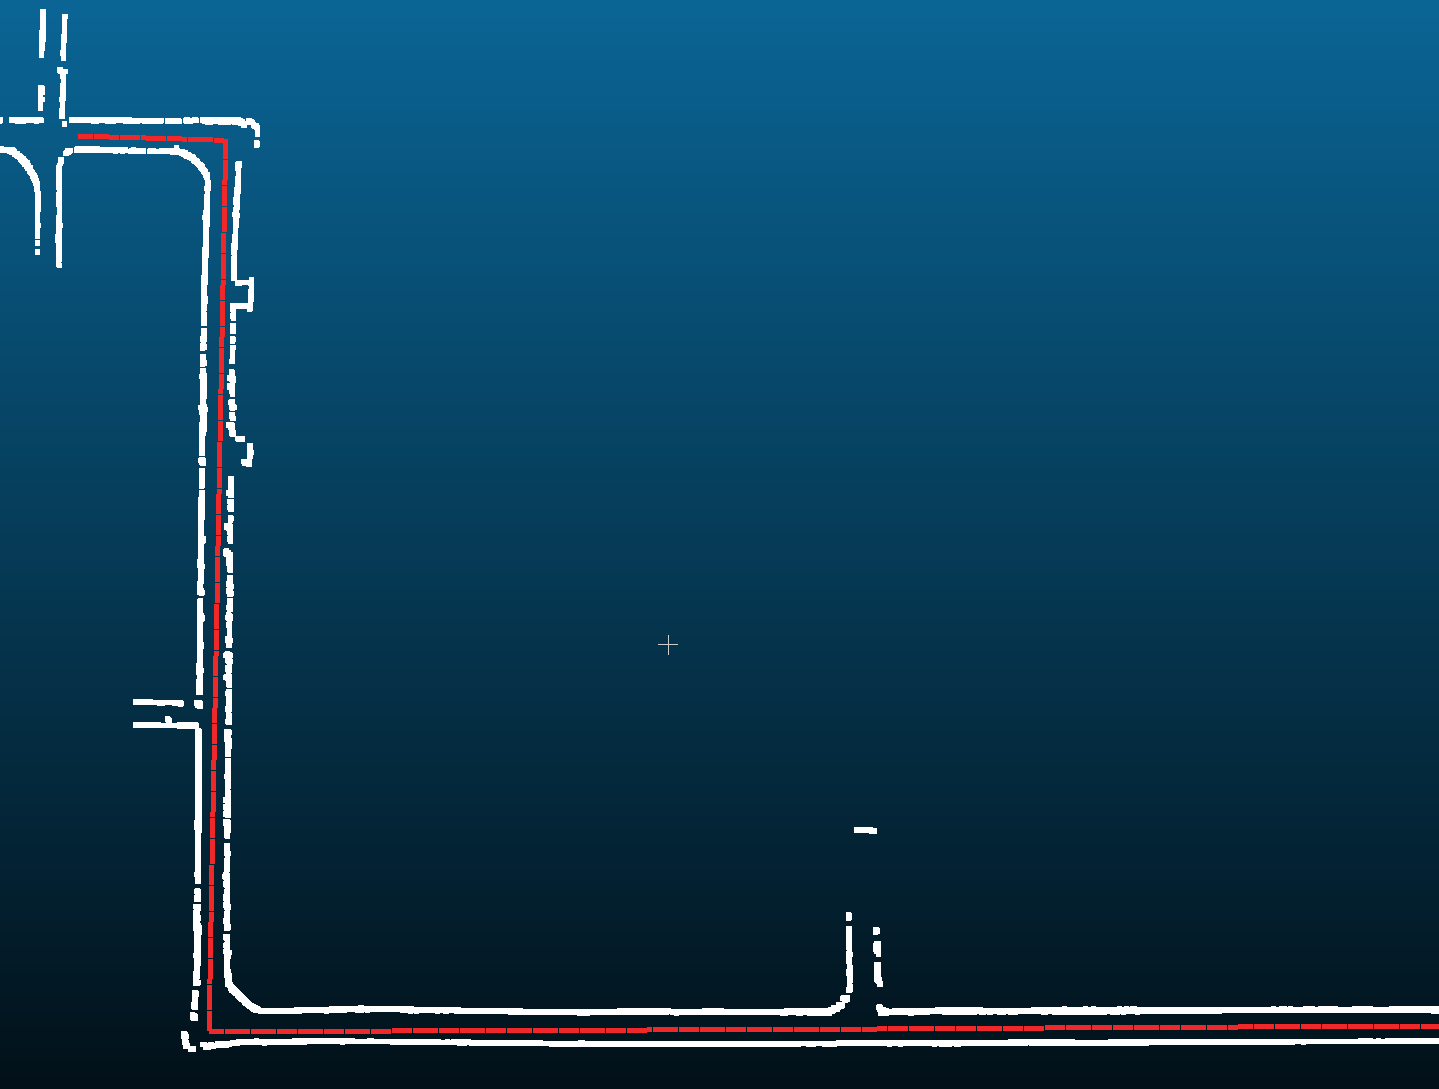
\includegraphics[width=0.92\textwidth]{figures/图4-3先验地图平面结构上的巷道中轴标注结果-1.png}
    \caption{先验地图平面结构上的巷道中轴标注结果}
    \label{fig:ch4_axis_centerline_prior}
\end{figure}

设矿井巷道中轴线由参数曲线 $\mathbf{c}(s)$ 表示，其中 $s$ 为弧长参数。考虑到中轴主要用于刻画巷道在水平平面内的延伸方向，本文以初始预测位置在 $XY$ 平面上的投影 $\mathbf{p}_{k,xy}^{0}$ 为基准，在中轴线平面投影 $\mathbf{c}_{xy}(s)$ 上搜索其最近投影点，即：
\begin{equation}
s_{k}^{\ast}
=
\arg \min_{s}
\left\|
\mathbf{p}_{k,xy}^{0}-\mathbf{c}_{xy}(s)
\right\|_{2}
\end{equation}

式中采用欧氏距离形式以便于表述，工程实现中等价地采用其平方形式以避免重复开方。由此得到当前时刻对应的中轴参考点：
\begin{equation}
\mathbf{c}_{k}
=
\mathbf{c}\left(s_{k}^{\ast}\right)
\end{equation}

以及对应的单位切向量：
\begin{equation}
\mathbf{u}_{k}
=
\frac{\dot{\mathbf{c}}\left(s_{k}^{\ast}\right)}
{\left\|\dot{\mathbf{c}}\left(s_{k}^{\ast}\right)\right\|_{2}}
\end{equation}

其中，$\mathbf{u}_{k}$ 表示当前时刻局部巷道轴向方向。

设两类平移观测分别为 $\hat{\mathbf{p}}_{k}^{f}$ 和 $\hat{\mathbf{p}}_{k}^{m}$。对于任一观测 $\hat{\mathbf{p}}_{k}^{j}$，其中 $j\in \{f,m\}$，定义其相对于中轴参考点的位移为：
\begin{equation}
\delta \mathbf{p}_{k}^{j}
=
\hat{\mathbf{p}}_{k}^{j}-\mathbf{c}_{k}
\end{equation}

则其轴向分量与非轴向分量可分别表示为：
\begin{equation}
\delta \mathbf{p}_{k,\parallel}^{j}
=
\left(\mathbf{u}_{k}^{\mathrm T}\delta \mathbf{p}_{k}^{j}\right)\mathbf{u}_{k}
\end{equation}
\begin{equation}
\delta \mathbf{p}_{k,\perp}^{j}
=
\delta \mathbf{p}_{k}^{j}-\delta \mathbf{p}_{k,\parallel}^{j}
\end{equation}

其中，$\delta \mathbf{p}_{k,\parallel}^{j}$ 表示对应的轴向投影向量，$\delta \mathbf{p}_{k,\perp}^{j}$ 表示去除轴向分量后剩余的非轴向偏移量。由此有：
\begin{equation}
\hat{\mathbf{p}}_{k}^{j}
=
\mathbf{c}_{k}
+\delta \mathbf{p}_{k,\parallel}^{j}
+\delta \mathbf{p}_{k,\perp}^{j}
\end{equation}

除中轴先验外，本文进一步由离线先验地图构建分层先验体素表，以形成面向方向化观测建模的统一结构先验。考虑到巷道横断面内不同空间区域对定位约束的贡献存在显著差异，本文依据空间点与稳定壁面边界之间的相对几何关系，将体素划分为轮廓区、过渡区和弱约束区，并分别赋予相应的先验权重。其中，轮廓区对应稳定壁面主体，用于表征最强的横断面结构支撑；过渡区对应壁面邻域，用于表征次级结构约束；弱约束区则对应巷道内部或结构属性不确定区域。该分层先验体素表并不直接参与位姿优化，而是作为方向化可信度建模的中间先验：在轴向方向上用于刻画局部观测的稳定性状态，在非轴向方向上用于评估地图观测与先验横断面结构之间的一致性。图~\ref{fig:ch4_prior_voxel_layer_generation} 给出了分层先验体素的空间分区结果示意。

\begin{figure}[htbp]
    \centering
    \fbox{
        \parbox{0.92\textwidth}{
            \centering
            分层先验体素空间分区结果占位图\\[4pt]
            左：先验地图局部结构区域；\quad
            右：分层先验体素分区结果，其中轮廓区、过渡区和弱约束区采用不同颜色显示
        }
    }
    \caption{分层先验体素空间分区结果示意图}
    \label{fig:ch4_prior_voxel_layer_generation}
\end{figure}

\subsection{轴向方向的自适应观测建模}

完成上述分解后，本文首先对轴向方向上的观测进行自适应建模。对于轴向方向而言，本文更关注载体沿巷道延伸方向的连续运动保持，但这种连续性并不意味着始终应单纯提高帧间观测权重。结合程序实现可以看出，轴向方向上的融合强度同时受到两类因素影响：其一是第~4.2 节得到的基础置信度及方向增益；其二是与当前场景状态相关的自适应修正项。前者给出双源观测的基础可信程度，后者则进一步刻画当前时刻轴向约束应被增强还是抑制。

具体地，设 $c_{k}^{f}$ 与 $c_{k}^{m}$ 分别表示帧间观测与地图观测的基础置信度，$\lambda_{\parallel}^{f}$ 与 $\lambda_{\parallel}^{m}$ 表示轴向方向增益系数。进一步引入地图侧轴向修正因子 $\alpha_{k,\parallel}^{m}$ 与帧间侧轴向修正因子 $\alpha_{k,\parallel}^{f}$，则轴向方向上的有效权重可写为：
\begin{equation}
\tilde{c}_{k,\parallel}^{f}
=
\lambda_{\parallel}^{f}\alpha_{k,\parallel}^{f}c_{k}^{f},
\qquad
\tilde{c}_{k,\parallel}^{m}
=
\lambda_{\parallel}^{m}\alpha_{k,\parallel}^{m}c_{k}^{m}
\end{equation}

其中，$\alpha_{k,\parallel}^{m}$ 与 $\alpha_{k,\parallel}^{f}$ 分别反映地图观测和帧间观测在轴向方向上的自适应调节结果。这样处理后，轴向权重不再仅由固定方向偏置给定，而是能够随当前巷道结构与局部观测状态变化而动态调整。

对于地图侧轴向修正，本文主要考虑巷道壁面结构对轴向定位可观性的支撑作用。矿井巷道虽然沿延伸方向存在较强重复性，但当当前位置附近具有更清晰的两侧壁面约束、更稳定的横断面起伏或更明显的几何边界时，地图配准在轴向方向上的参考意义也会相应增强。为此，本文定义结构约束强度指标 $r_{k}^{w}\in[0,1]$，用于衡量当前位置附近壁面结构对轴向估计的支撑程度，并据此构造地图侧轴向修正因子：
\begin{equation}
\alpha_{k,\parallel}^{m}
=
\varphi_{m}\!\left(r_{k}^{w}\right)
\end{equation}

其中，$\varphi_{m}(\cdot)$ 为单调非减映射函数，并在有界区间内取值。当局部壁面结构清晰、地图配准收敛稳定时，$\alpha_{k,\parallel}^{m}$ 适度增大，以增强地图观测在轴向方向上的约束作用；当结构支撑不足或地图观测质量较弱时，则保持其中性取值，避免将不可靠的地图信息过度引入轴向估计。

对于帧间侧轴向修正，本文主要考虑当前局部观测与先验环境之间的一致性稳定程度。若当前帧在先验地图中持续出现较多难以解释的局部结构，则意味着场景中可能存在设备停放、堆料遮挡或局部工况变化，此时仅依赖短时帧间连续性容易在轴向方向上传递瞬时扰动。为此，本文进一步利用分层先验体素表刻画当前局部观测相对于先验环境的稳定偏离程度，并引入局部观测稳定性指标 $r_{k}^{s}\in[0,1]$：
\begin{equation}
r_{k}^{s}
=
r_{k}^{u}r_{k}^{su}
\end{equation}

其中，$r_{k}^{u}$ 表示当前帧在地图观测位姿下落入弱约束区或先验未支撑体素的比例，$r_{k}^{su}$ 表示该类异常体素在滑动时间窗口内的持续出现比例。前者反映当前时刻局部观测相对于先验结构的即时偏离程度，后者反映该偏离是否具有时间上的持续性。由此，同一分层先验体素表不仅用于描述横断面稳定结构，也可用于表征轴向方向上的局部观测稳定状态。进一步地，构造帧间侧轴向修正因子：
\begin{equation}
\alpha_{k,\parallel}^{f}
=
\varphi_{f}\!\left(r_{k}^{s}\right)
\end{equation}

其中，$\varphi_{f}(\cdot)$ 为分段有界映射函数，其作用是在中性点附近保持平缓，而在观测稳定性明显变化时对帧间轴向权重进行适度调节。这样可使帧间观测在常规工况下继续承担轴向连续性保持作用，而在局部扰动持续出现时抑制其对融合结果的过强牵引。

综上，本文轴向自适应建模的核心并非简单预设“帧间强、地图弱”的固定关系，而是在中轴分解基础上，将基础置信度、方向增益以及场景相关修正因子共同纳入轴向权重建模过程。至此，轴向自适应观测由中轴参考点 $\mathbf{c}_{k}$、两类轴向分量 $\delta \mathbf{p}_{k,\parallel}^{f}$、$\delta \mathbf{p}_{k,\parallel}^{m}$ 以及对应的轴向有效权重 $\tilde{c}_{k,\parallel}^{f}$、$\tilde{c}_{k,\parallel}^{m}$ 共同构成。

\subsection{基于分层先验体素一致性的非轴向观测建模}

在完成轴向方向建模后，本文进一步考虑非轴向方向上的结构约束构造。与轴向方向更强调局部连续性不同，非轴向方向的定位可观性主要来源于巷道横断面中的稳定壁面及边界结构。然而，矿井巷道内常存在设备、车辆、堆料等半静态变化物体，局部点云观测会随工况变化而发生扰动，因此仅依赖地图配准得分仍难以充分刻画地图观测在非轴向方向上的真实可靠性。基于此，本文利用上述分层先验体素表，对地图观测实施基于结构一致性的非轴向自适应修正。

设由离线先验地图构建得到的分层先验体素集合记为 $\mathcal{V}$，体素边长为 $l_v$。对于任意空间点 $\mathbf{p}=[x,y,z]^{\mathrm T}$，其对应的体素索引可表示为：
\begin{equation}
\nu(\mathbf{p})
=
\left[
\left\lfloor \frac{x}{l_v}\right\rfloor,
\left\lfloor \frac{y}{l_v}\right\rfloor,
\left\lfloor \frac{z}{l_v}\right\rfloor
\right]^{\mathrm T}
\end{equation}

其中，$\nu(\cdot)$ 表示体素索引映射算子。记 $\omega\!\left(\nu(\mathbf{p})\right)\in[0,1]$ 为对应体素的先验权重：当空间点落入轮廓区时取较大值，落入过渡区时取次级值，落入弱约束区时取较小值；若对应索引不在有效体素表中，则取 $0$。由此可将横断面结构约束强弱统一编码到体素查询结果中。

设当前帧点云 $\mathcal{P}_{k}=\{\mathbf{p}_{k,i}\}_{i=1}^{N_k}$ 在地图观测 $\hat{\mathbf{T}}_{k}^{m}$ 下被变换到全局坐标系后的点为：
\begin{equation}
\mathbf{p}_{k,i}^{g,m}
=
\hat{\mathbf{T}}_{k}^{m}\odot \mathbf{p}_{k,i}
=
\mathbf{R}\left(\hat{\mathbf{q}}_{k}^{m}\right)\mathbf{p}_{k,i}
+\hat{\mathbf{p}}_{k}^{m}
\end{equation}

其中，$\odot$ 表示刚体变换对点的作用，$\hat{\mathbf{p}}_{k}^{m}$ 和 $\hat{\mathbf{q}}_{k}^{m}$ 分别表示地图观测的平移与姿态分量。进一步地，当前帧在地图观测位姿下与分层先验体素表之间的加权一致性可表示为：
\begin{equation}
r_{k}^{v}
=
\frac{1}{N_k}\sum_{i=1}^{N_k}\omega\!\left(\nu\left(\mathbf{p}_{k,i}^{g,m}\right)\right)
\end{equation}

其中，$r_{k}^{v}\in [0,1]$ 反映了当前帧点云与分层先验体素表之间的整体一致性程度。当 $r_{k}^{v}$ 较高时，说明地图观测所对应的点云位置与先验横断面结构具有较好一致性，且更多落入轮廓区和过渡区；反之，则说明地图观测可能存在一定偏差，尤其是在结构重复、局部错配或横断面约束不足的情况下，其可靠性应进一步降低。

由于矿井巷道沿轴向方向具有较强的几何重复性，体素命中统计对轴向漂移的辨识能力有限，而对横断面方向上的位置偏差更为敏感。因此，本文仅利用体素命中一致性修正地图观测在非轴向方向上的置信度，并采用有界线性映射将体素命中率转换为一致性系数：
\begin{equation}
\eta_{k}^{v}
=
\eta_{\min}
+\left(1-\eta_{\min}\right)
\mathrm{clip}
\left(
\frac{r_{k}^{v}-r_{\mathrm{bad}}}{r_{\mathrm{good}}-r_{\mathrm{bad}}},
0,1
\right)
\end{equation}

其中，$r_{\mathrm{good}}$ 与 $r_{\mathrm{bad}}$ 分别表示体素命中率较高和较低时的参考边界，$\eta_{\min}$ 表示一致性系数下界，$\mathrm{clip}(x,0,1)$ 表示将变量 $x$ 截断到区间 $[0,1]$ 内。由此可见，命中率越高，对应的一致性系数越大；当命中率较低时，其取值不会低于 $\eta_{\min}$。

在此基础上，地图观测在非轴向方向上的修正置信度可定义为：
\begin{equation}
\bar{c}_{k,\perp}^{m}
=
c_{k}^{m}\eta_{k}^{v}
\end{equation}

其中，$c_{k}^{m}$ 为上一节依据地图配准得分得到的基础置信度，$\bar{c}_{k,\perp}^{m}$ 为经先验体素一致性修正后的非轴向置信度。

在非轴向方向上，帧间观测同样提供局部连续性信息，因此本文进一步定义非轴向方向上的有效权重为：
\begin{equation}
\tilde{c}_{k,\perp}^{f}
=
\lambda_{\perp}^{f}c_{k}^{f},
\qquad
\tilde{c}_{k,\perp}^{m}
=
\lambda_{\perp}^{m}\bar{c}_{k,\perp}^{m}
\end{equation}

其中，$\lambda_{\perp}^{f}$ 与 $\lambda_{\perp}^{m}$ 为非轴向方向增益系数。通常取 $\lambda_{\perp}^{m}>\lambda_{\perp}^{f}$，以体现非轴向方向更侧重稳定地图结构约束的设计思想。至此，非轴向自适应观测由两类非轴向分量 $\delta \mathbf{p}_{k,\perp}^{f}$、$\delta \mathbf{p}_{k,\perp}^{m}$ 以及对应的非轴向有效权重 $\tilde{c}_{k,\perp}^{f}$、$\tilde{c}_{k,\perp}^{m}$ 共同构成。

\section{基于轴向与非轴向观测的加权融合估计}

经过上一节的分解与自适应建模，本文已经分别获得轴向观测和非轴向观测。前者强调巷道延伸方向上的局部连续运动信息，后者强调横断面方向上的稳定结构约束。基于这一并列建模结果，本节进一步对两类观测实施统一加权融合，得到最终位姿估计。

\subsection{平移分量融合}

设 $\tilde{c}_{k,\parallel}^{f}$、$\tilde{c}_{k,\parallel}^{m}$ 为轴向方向上的两类有效权重，$\tilde{c}_{k,\perp}^{f}$、$\tilde{c}_{k,\perp}^{m}$ 为非轴向方向上的两类有效权重，则可分别定义帧间观测在轴向与非轴向融合中的归一化权重：
\begin{equation}
\alpha_{k,\parallel}
=
\frac{\tilde{c}_{k,\parallel}^{f}}
{\tilde{c}_{k,\parallel}^{f}+\tilde{c}_{k,\parallel}^{m}}
\end{equation}
\begin{equation}
\alpha_{k,\perp}
=
\frac{\tilde{c}_{k,\perp}^{f}}
{\tilde{c}_{k,\perp}^{f}+\tilde{c}_{k,\perp}^{m}}
\end{equation}

于是，轴向分量与非轴向分量的融合结果可分别写为：
\begin{equation}
\hat{\delta \mathbf{p}}_{k,\parallel}
=
\left(1-\alpha_{k,\parallel}\right)\delta \mathbf{p}_{k,\parallel}^{m}
+\alpha_{k,\parallel}\delta \mathbf{p}_{k,\parallel}^{f}
\end{equation}
\begin{equation}
\hat{\delta \mathbf{p}}_{k,\perp}
=
\left(1-\alpha_{k,\perp}\right)\delta \mathbf{p}_{k,\perp}^{m}
+\alpha_{k,\perp}\delta \mathbf{p}_{k,\perp}^{f}
\end{equation}

由此可得最终融合位置估计：
\begin{equation}
\hat{\mathbf{p}}_{k}
=
\mathbf{c}_{k}
+\hat{\delta \mathbf{p}}_{k,\parallel}
+\hat{\delta \mathbf{p}}_{k,\perp}
\end{equation}

由此可见，上一节完成的是轴向与非轴向观测的分解与建模，而本节完成的是在统一框架下对两类观测进行加权汇合。

\subsection{姿态分量融合}

对于姿态分量，本文不再进行轴向分解，而是仍依据两类观测的整体置信度进行融合。设帧间观测与地图观测对应的姿态分别为 $\hat{\mathbf{q}}_{k}^{f}$ 和 $\hat{\mathbf{q}}_{k}^{m}$，则定义帧间姿态观测的融合系数为：
\begin{equation}
\alpha_{k}^{q}
=
\frac{c_{k}^{f}}{c_{k}^{f}+c_{k}^{m}}
\end{equation}

进一步地，利用四元数球面线性插值可得到最终姿态估计：
\begin{equation}
\hat{\mathbf{q}}_{k}
=
\mathrm{Slerp}
\left(
\hat{\mathbf{q}}_{k}^{m},
\hat{\mathbf{q}}_{k}^{f},
\alpha_{k}^{q}
\right)
\end{equation}

其中，$\mathrm{Slerp}(\cdot)$ 表示四元数球面线性插值算子。最终，当前时刻的融合位姿估计可表示为：
\begin{equation}
\hat{\mathbf{T}}_{k}
=
\begin{bmatrix}
\mathbf{R}\left(\hat{\mathbf{q}}_{k}\right) & \hat{\mathbf{p}}_{k}\\
\mathbf{0}^{\mathrm T} & 1
\end{bmatrix}
\end{equation}

上述融合在轴向方向保持局部运动连续性，在非轴向方向强化先验地图约束，从而在统一位姿估计中兼顾两类方向观测的作用。

\section{实验验证与结果分析}

\subsection{实验数据、对比方案与评价依据}

为验证本文所提出基于先验地图约束的轴向-非轴向分解与融合定位方法在实际先验条件下的有效性，本文在真实地下矿井数据集和 Gazebo 仿真数据集上开展实验。与第三章面向离线建图质量的验证目标不同，本章关注的是第三章构建所得先验地图对在线定位的支撑能力，因此两组实验均固定采用第 3 章优化后得到的先验地图作为地图配准参考，并在统一先验条件下比较不同定位方法的表现。

具体而言，对于真实地下矿井场景，本文采用第三章基于真实井下采集数据优化得到的先验地图，并选取独立采集的井下运行序列作为定位输入，从而检验所提方法对真实井下长距离运行、结构重复和局部扰动的适应能力。对于 Gazebo 仿真场景，本文同样以前述建图流程生成的优化后地图作为定位先验，并结合仿真系统输出的真值位姿进行误差评估。通过这一实验设置，可在更贴近工程应用的先验条件下分析定位模块的轨迹误差、稳定性和融合效果。

两组实验统一采用相同的点云预处理流程，包括车体点剔除、离群点滤除和体素下采样。对于真实地下矿井场景，由于目前缺少与定位序列严格对齐的独立参考轨迹，因此主要结合累计点云与先验地图之间的一致性进行辅助评价；对于 Gazebo 仿真数据集，则仍以仿真系统输出的真值轨迹作为误差评估基准。除实验场景不同外，两组实验在初始化方式、地图调用方式和双源配准流程上保持一致，以保证对比结果能够直接反映所提方法在统一先验条件下的定位性能。

为体现所提方法中非轴向先验体素修正以及轴向-非轴向分解与融合机制的作用，本文设置以下对比方案：

（1）HDL-Location：公开的先验地图定位基线方法。

（2）Uniform-Weight Fusion：Fast-GICP 结果一方面为 NDT 地图配准提供初值，另一方面作为帧间观测参与最终位姿融合；但不引入先验体素命中修正和轴向/非轴向差异化处理，而是采用统一权重对 Fast-GICP 与 NDT 结果进行整体融合。

（3）Axis-Decomposed Fusion (Proposed)：Fast-GICP 结果同样用于为 NDT 地图配准提供初值，并在最终位姿估计中与 NDT 结果共同参与融合；同时在地图观测侧引入先验体素一致性修正，并结合巷道中轴对 Fast-GICP 与 NDT 的平移观测实施轴向分解与差异化融合。

实验中使用的主要参数包括点云下采样分辨率、先验体素边长、体素命中率阈值以及轴向与非轴向方向增益系数等。考虑到真实井下环境与仿真场景在点云密度、巷道尺度和局部扰动程度上存在差异，本文在保持定位框架一致的前提下，对少量阈值参数进行了与场景尺度相匹配的设定。第四章实验的主要参数配置如表~\ref{tab:ch4_exp_params} 所示。

\begin{table}[htbp]
    \centering
    \caption{第四章定位实验主要参数配置}
    \label{tab:ch4_exp_params}
    \small
    \renewcommand{\arraystretch}{1.15}
    \begin{tabular}{p{6.2cm}p{4.0cm}}
        \toprule
        参数名称 & 取值 \\
        \midrule
        点云下采样分辨率 & 待补充 \\
        NDT 地图分辨率 & 待补充 \\
        先验体素边长 $l_v$ & 待补充 \\
        命中率低阈值 $r_{\mathrm{bad}}$ & 待补充 \\
        命中率高阈值 $r_{\mathrm{good}}$ & 待补充 \\
        一致性系数下界 $\eta_{\min}$ & 待补充 \\
        轴向帧间增益 $\lambda_{\parallel}^{f}$ & 待补充 \\
        轴向地图增益 $\lambda_{\parallel}^{m}$ & 待补充 \\
        非轴向帧间增益 $\lambda_{\perp}^{f}$ & 待补充 \\
        非轴向地图增益 $\lambda_{\perp}^{m}$ & 待补充 \\
        \bottomrule
    \end{tabular}
\end{table}

本章评价方法总体沿用第 2 章和第 3 章中的评价思路，不再重复展开指标定义。对于能够提供严格对齐真值轨迹的 Gazebo 仿真数据集，本文采用绝对位姿误差（APE）对不同方法的定位精度进行定量比较，并以均方根误差、平均误差和中位数误差作为主要统计量；对于缺少独立参考轨迹的真实地下矿井数据集，则采用基于先验地图的 MapEval 指标对累计定位结果进行辅助评价。

因此，本章的评价重点不在于重新定义评价指标，而在于分析在第三章先验地图条件下，不同定位方法在仿真场景中的轨迹精度差异，以及在真实井下场景中的几何一致性与结构保持能力。

\subsection{Gazebo 仿真场景定位结果分析}

Gazebo 仿真数据集由本文搭建的矿井巷道仿真环境生成，能够提供与激光时间戳严格对齐的机器人真值轨迹。本节固定采用第三章建图流程在 Gazebo 场景中生成的优化后先验地图作为定位参考，并在统一先验条件下比较不同定位策略的轨迹精度差异。相比真实地下矿井数据集，仿真环境能够在控制变量条件下更清晰地分析不同定位策略的精度差异，因此适合用于验证本文方法在实际建图先验条件下的定位性能。

图~\ref{fig:ch4_gazebo_compare} 建议汇总展示 Gazebo 仿真数据集上的轨迹对比结果与绝对误差分析结果。其中，子图（a）用于联合展示不同方法与真值轨迹的俯视叠加结果以及绝对轨迹误差对比结果；子图（b）用于并排展示位置与姿态分量随时间的变化对比。图中图例可统一标注为 Ground Truth、HDL-Location、Uniform-Weight Fusion 和 Axis-Decomposed Fusion (Proposed)。

\begin{figure}[p]
    \centering
    \begin{minipage}[t]{0.48\linewidth}
        \centering
        \IfFileExists{figures/图4.5(a-1).png}{
            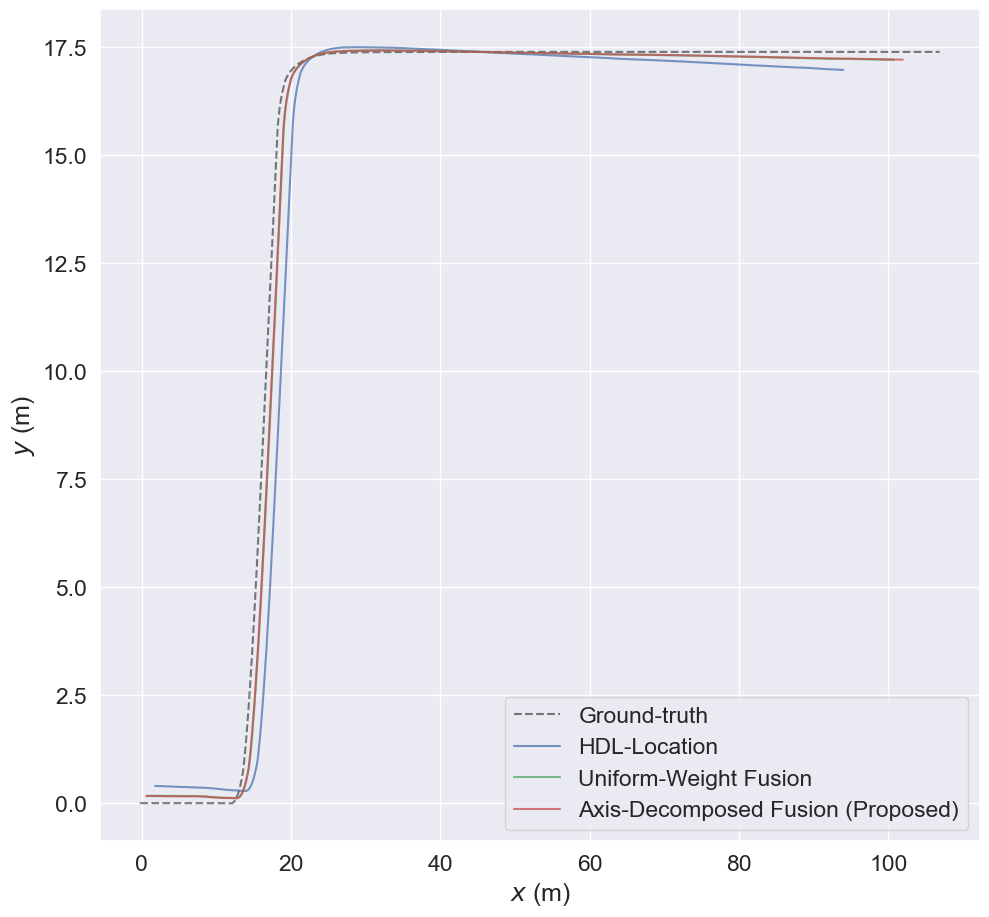
\includegraphics[width=\linewidth]{figures/图4.5(a-1).png}
        }{
            \fbox{
                \parbox{0.92\linewidth}{
                    \centering
                    图 4.5（a-1）轨迹对比图占位图\\[4pt]
                    建议内容：Ground Truth、HDL-Location、Uniform-Weight Fusion、\\[2pt]
                    Axis-Decomposed Fusion (Proposed) 的俯视轨迹叠加结果。
                }
            }
        }
    \end{minipage}
    \hfill
    \begin{minipage}[t]{0.48\linewidth}
        \centering
        \IfFileExists{figures/图4.5(d).png}{
            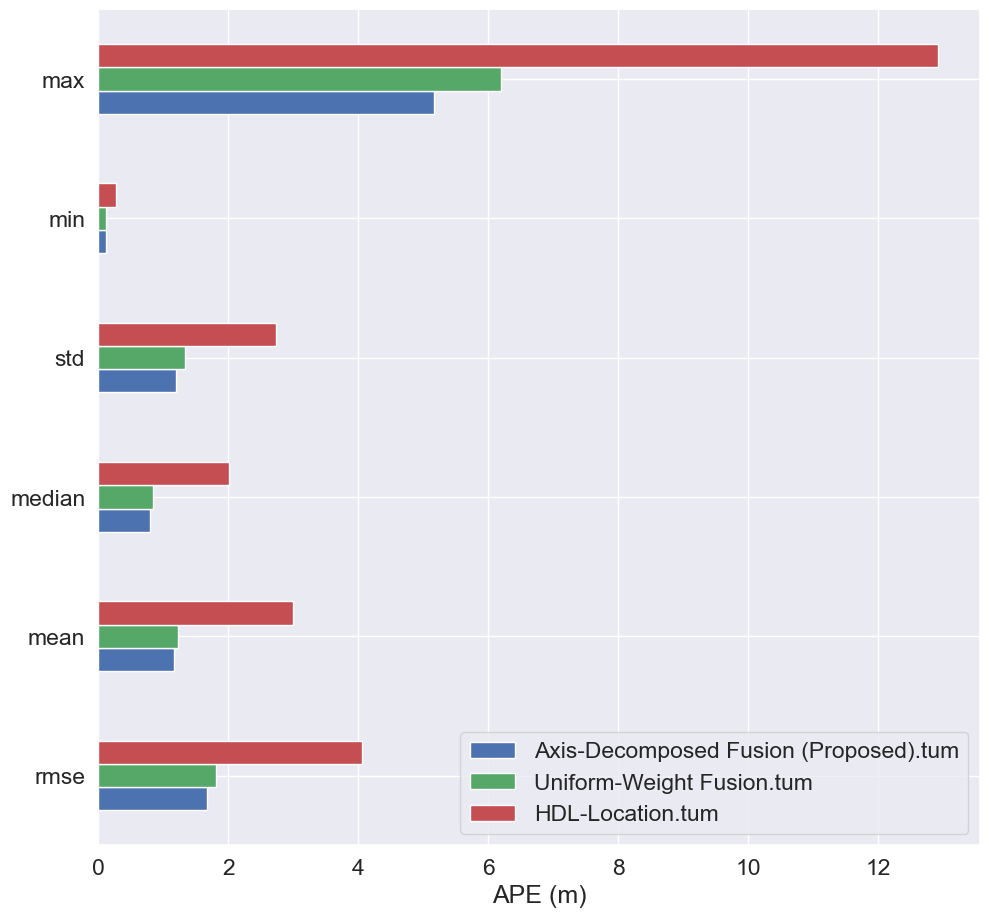
\includegraphics[width=\linewidth]{figures/图4.5(d).png}
        }{
            \fbox{
                \parbox{0.92\linewidth}{
                    \centering
                    图 4.5（a-2）绝对轨迹误差对比图占位图\\[4pt]
                    建议内容：不同方法 APE 曲线、箱线图或统计结果可视化。
                }
            }
        }
    \end{minipage}\\[1pt]
    （a）轨迹与绝对轨迹误差对比\\[3pt]
    \begin{minipage}[t]{0.48\linewidth}
        \centering
        \IfFileExists{figures/图4.5(b).png}{
            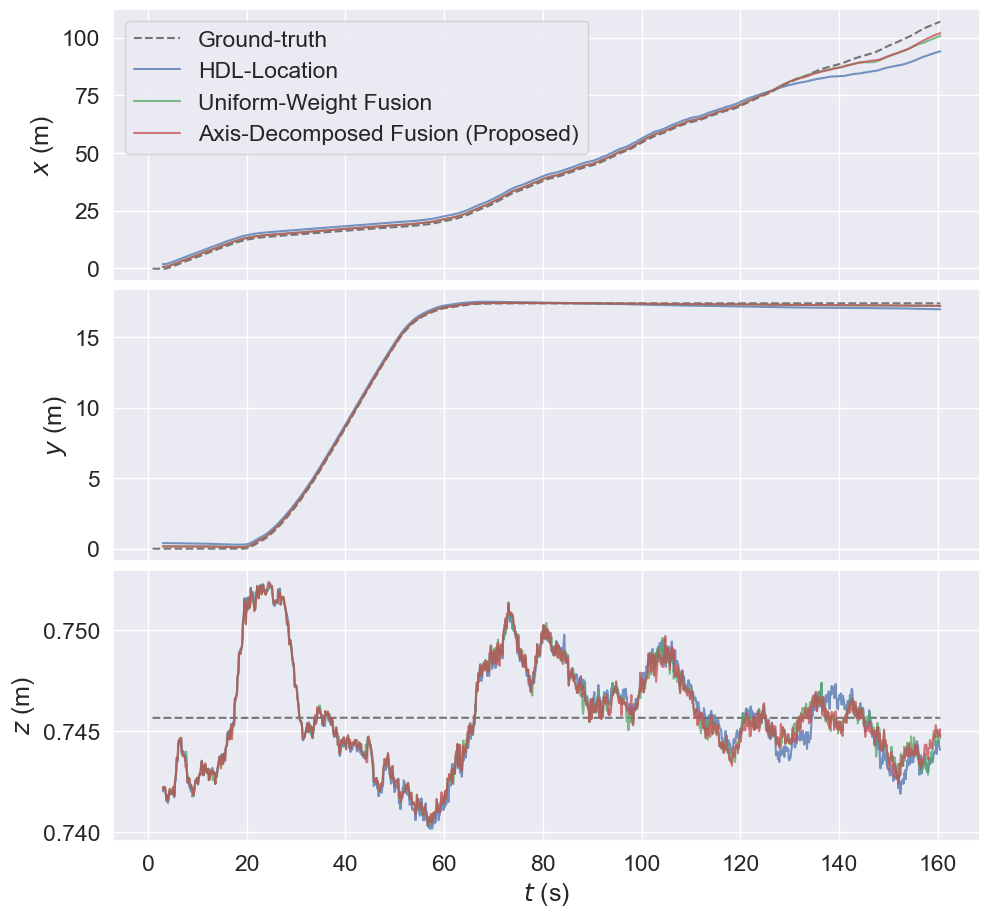
\includegraphics[width=\linewidth]{figures/图4.5(b).png}
        }{
            \fbox{
                \parbox{0.92\linewidth}{
                    \centering
                    XYZ 方向绝对误差图占位图
                }
            }
        }
    \end{minipage}
    \hfill
    \begin{minipage}[t]{0.48\linewidth}
        \centering
        \IfFileExists{figures/图4.5(c).png}{
            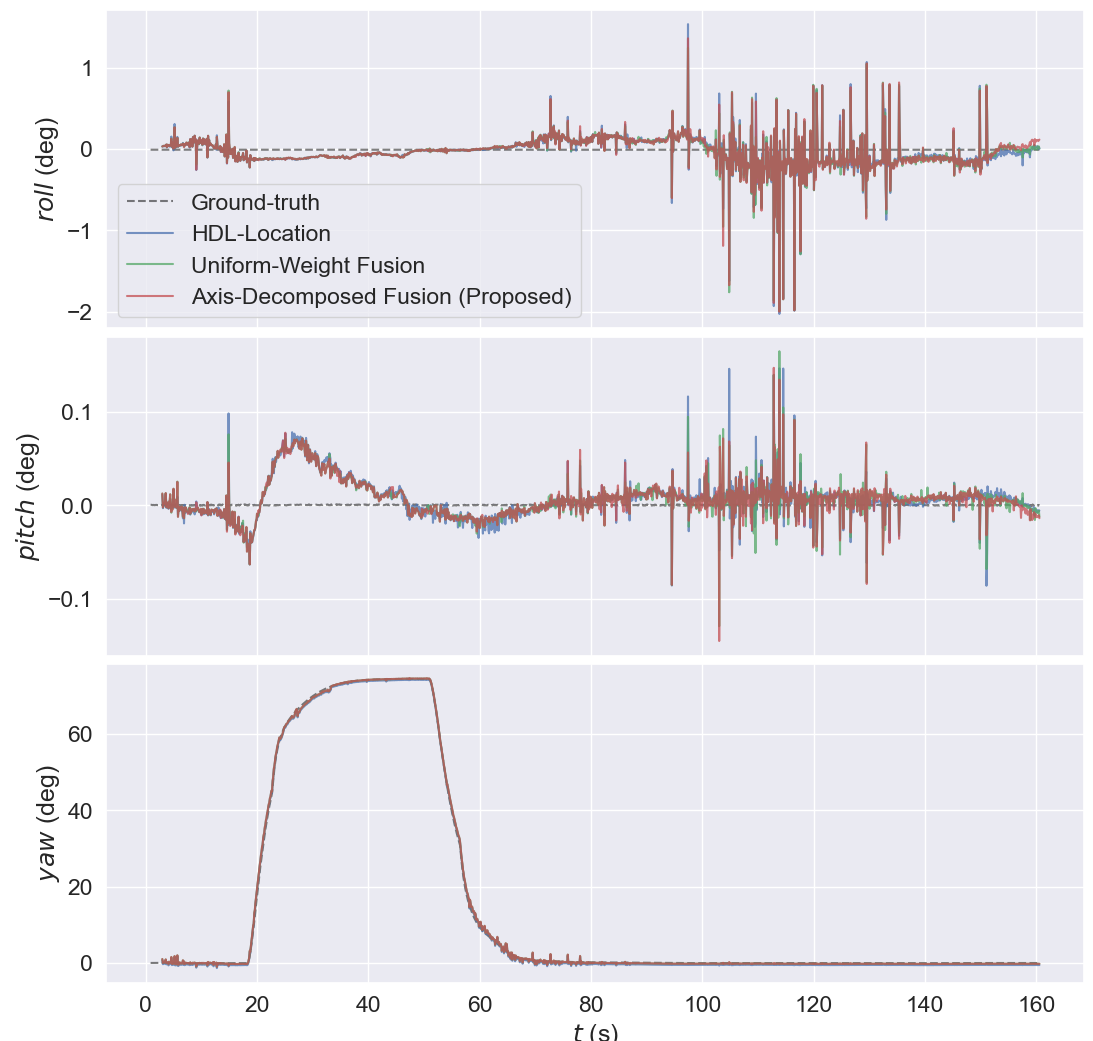
\includegraphics[width=\linewidth]{figures/图4.5(c).png}
        }{
            \fbox{
                \parbox{0.92\linewidth}{
                    \centering
                    RPY 方向绝对误差图占位图
                }
            }
        }
    \end{minipage}\\[1pt]
    （b）位置与姿态分量对比
    \caption{Gazebo 仿真数据集上的轨迹与绝对误差对比}
    \label{fig:ch4_gazebo_compare}
\end{figure}

Gazebo 仿真数据集上的定量结果如表~\ref{tab:ch4_gazebo_result} 所示。由于该数据集能够提供精确真值轨迹，因此更适合从绝对误差角度比较不同方法的定位精度。实验结果表明，公开基线 HDL-Location 的误差相对较大；Uniform-Weight Fusion 较其有所改善，但由于未区分轴向和非轴向约束特性，其整体精度仍不及本文方法。

Axis-Decomposed Fusion (Proposed) 在 Gazebo 仿真数据集上表现出优于 HDL-Location 和 Uniform-Weight Fusion 的误差水平。这说明轴向分解能够在巷道延伸方向上更合理地保留帧间观测带来的局部连续运动信息，而先验体素约束则有助于提升地图观测在横断面方向上的可靠性判别能力，从而使非轴向位置更稳定地收敛到正确的巷道结构范围内。综合来看，本文方法进一步体现了差异化融合策略相较于简单统一加权方式的有效性。

\begin{table}[htbp]
    \centering
    \caption{Gazebo 仿真数据集上基于第三章优化后地图的定位结果对比}
    \label{tab:ch4_gazebo_result}
    \small
    \renewcommand{\arraystretch}{1.15}
    \begin{tabular}{cccc}
        \toprule
        方法 & \shortstack{均方根误差\\(m)} & \shortstack{平均误差\\(m)} & \shortstack{中位数误差\\(m)} \\
        \midrule
        HDL-Location & 6.723 & 6.220 & 5.742 \\
        Uniform-Weight Fusion & 3.248 & 2.973 & 2.723 \\
        \shortstack{Axis-Decomposed Fusion\\(Proposed)} & \textbf{2.900} & \textbf{2.757} & \textbf{2.514} \\
        \bottomrule
    \end{tabular}
\end{table}

\subsection{真实地下矿井场景定位结果分析}

真实地下矿井数据集采集于陕西大海则煤矿井下巷道，相关场景与采集条件已在第三章中给出。与第三章直接面向建图质量评估不同，本节关注的是优化后先验地图支持下的定位性能，因此实验中固定采用第三章构建得到的真实地下矿井先验地图，并输入独立采集的井下运行序列，分析不同定位方法在同一先验地图条件下的性能差异。该场景具有轨迹长、结构重复强和局部工况扰动明显等特点，能够较好地检验定位方法在真实井下环境中的连续运行能力。

图~\ref{fig:ch4_realmine_compare} 建议展示不同方法在真实地下矿井场景中的定位结果对比，可采用“累计定位结果叠加图 + 局部典型区域放大图”的形式。全局结果图用于比较长距离运行下不同方法的整体一致性，局部放大图则重点展示长直巷道、转弯区域以及结构重复区域的差异。

\begin{figure}[htbp]
    \centering
    \fbox{
        \parbox{0.92\linewidth}{
            \centering
            此处插入真实地下矿井数据集定位结果对比图\\[4pt]
            建议包含：各对比方法与本文方法的全局/局部对比结果。
        }
    }
    \caption{真实地下矿井数据集上的定位结果对比}
    \label{fig:ch4_realmine_compare}
\end{figure}

由于目前缺少与真实地下矿井定位序列严格对应的独立参考轨迹，本节不再给出基于轨迹误差统计的定量对比表。为对不同方法在真实井下场景中的定位结果进行辅助分析，本文进一步参照第三章的 MapEval 指标，对不同定位方法生成的累计点云结果进行量化比较，结果如表~\ref{tab:ch4_realmine_mapeval} 所示。参考第三章中的指标定义，本文仍以 AWD 作为绝对几何一致性的核心指标，以 COM 作为覆盖完整性的补充指标，并结合 CD 与 AC 分析定位结果与第三章优化后先验地图之间的整体距离误差和点级误差。需要说明的是，当前 MapEval 实现输出中的 VMD 项对应表中的 AWD。由表中结果可知，Uniform-Weight Fusion 相较于 HDL-Location 已在 AWD、COM 和 CD 上有所改善；相比之下，Axis-Decomposed Fusion (Proposed) 在 COM 和 CD 上表现更优，说明本文方法在真实井下场景下生成的累计点云与第三章优化后先验地图具有更好的一致性和完整性。

\begin{table}[htbp]
    \centering
    \caption{基于第三章优化后先验地图的真实地下矿井定位结果辅助量化对比}
    \label{tab:ch4_realmine_mapeval}
    \small
    \begin{tabular}{cccccc}
        \toprule
        数据集 & 方法 & \shortstack{绝对一致性\\AWD$\downarrow$ (m)} & \shortstack{完整性\\COM$\uparrow$ (-)} & \shortstack{Chamfer 距离\\CD$\downarrow$ (m)} & \shortstack{准确性\\AC$\downarrow$ (m)} \\
        \midrule
        \multirow{3}{*}{真实地下矿井数据集} & HDL-Location & \textbf{0.378} & 0.974 & 0.688 & \textbf{0.296} \\
         & Uniform-Weight Fusion & 0.378 & 0.975 & 0.681 & 0.298 \\
         & \shortstack{Axis-Decomposed Fusion\\(Proposed)} & 0.379 & \textbf{0.995} & \textbf{0.477} & 0.301 \\
        \bottomrule
    \end{tabular}
\end{table}

综合两类场景实验可以看出，在统一采用第三章优化后地图作为定位先验的条件下，真实地下矿井场景下的辅助量化结果能够反映所提方法在复杂工况下的稳定性优势，而 Gazebo 仿真数据集则体现了本文方法在统一先验条件下的轨迹精度优势。二者相互补充，共同验证了所提方法对实际建图先验的适用性，也说明第三章构建的先验地图能够有效支撑第四章定位方法的运行。

\section{本章小结}

本章面向矿井巷道场景中定位约束方向性不均衡的问题，提出了一种基于先验地图约束的轴向-非轴向分解与融合定位方法。首先，构建了由 IMU 初始预测、帧间配准观测和地图配准观测组成的递进式观测建模框架，为后续融合提供基础位姿观测与置信信息。随后，围绕巷道轴向和非轴向方向分别建立观测分解与约束建模，其中轴向方向依托中轴先验保持局部连续性，非轴向方向利用先验体素命中统计修正地图观测可靠性。最后，依据两类观测的权重关系进行加权融合，得到最终位姿估计结果。

通过上述建模，本文方法在保持局部运动连续性的同时，进一步利用了先验地图在横断面方向上的稳定结构约束，从而能够更好地适应矿井巷道场景中常见的结构重复、局部退化和观测波动等问题。下一章将在此基础上进一步研究大尺度场景下高精先验地图的组织、调用与动态管理方法。
